%===================================================================================
% Chapter: Análisis Experimental
%===================================================================================
\chapter{Análisis Experimental}\label{chapter:experiments}
\addcontentsline{toc}{chapter}{Análisis Experimental}

Este capítulo se centra en la descripción del los detalles de la implementación de las propuestas descritas para la extracción de entidades y relaciones.
Se explican las configuraciones de los exprimentos realizados y el conjunto de técnicas experimentales empleadas, se muestran los resultados de dicho estudio y se someten los mismo a una posterior discusión.

\section{Marco Experimental}

El desarrollo de los experimentos de este trabajo se enmarca en el evento \textit{eHealth Knowledge Discovery Challenge}, en sus ediciones de 2019 y 2020.
En la misma, los problemas de extracción de entidades y relaciones están organizados en dos tareas.

\begin{description}
	\item[Tarea A:] Extracción y clasificación de entidades.
	Dada una lista de documentos del ámbito del eHealth en idioma español, el objetivo de	esta tarea es identificar las entidades por documento y clasificarlas según el tipo de concepto que representan~(\texttt{Concept}, \texttt{Action}, \texttt{Predicate} o \texttt{Reference}).
	Las palabras clave son todos los conceptos relevantes~(de una o múltiples palabras) que representan elementos
	semánticamente importantes en la oración.
	La figura \ref{fig:entites_ex} muestra las palabras clave relevantes que aparecen en un conjunto de oraciones de ejemplo.
	
	La entrada de la Tarea A es un documento de texto con una oración	por línea. Todas las oraciones han sido tokenizadas a nivel de palabra~(o sea, signos de puntuación, paréntesis, etc., son separados del texto que los rodea).
	La salida de la Tarea A es una lista de extensiones de texto, identificadas por secuencias de tuplas \texttt{<INICIO,FIN>}, en las que se mencionan conceptos.
	Estas instancias específicas de conceptos son llamadas entidades y se les asigna un identificador numérico.
	
	\item[Tarea B:] Extracción de relaciones.
	La Tarea B extiende los resultados de la Tarea A, a partir de enlazar las palabras claves previamente detectadas y etiquetadas en cada oración.
	El propósito de esta tarea es reconocer todas las relaciones semánticas relevantes entre los conceptos identificados.
	Ocho de las trece relaciones semánticas presentes en el conjunto de datos pueden ser observadas en la figura \ref{fig:relations_ex}.
		
	La entrada de la Tarea B es un documento de texto con una oración	por línea, y una colección de entidades numeradas y etiquetadas.
	La salida de la Tarea B es una lista de tuplas de la forma \texttt{<id1,id2,rel>} que denota la ocurrencia de una relación de tipo \texttt{rel}, con origen en la entidad con identificador \texttt{id1}, y destino en \texttt{id2}.
	
\end{description} 
	
\begin{figure}[h!]
	\centering
	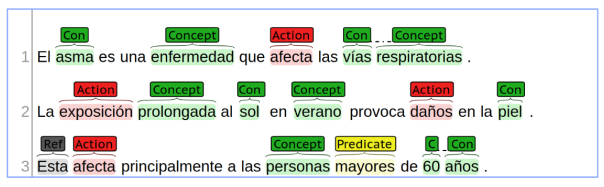
\includegraphics[width=0.9\linewidth]{Graphics/entities.png}
	\caption{Anotación de las entidades relevantes y sus respectivas clases en un conjunto de oraciones de ejemplo.} \label{fig:entites_ex}
\end{figure}

\begin{figure}[h!]
	\centering
	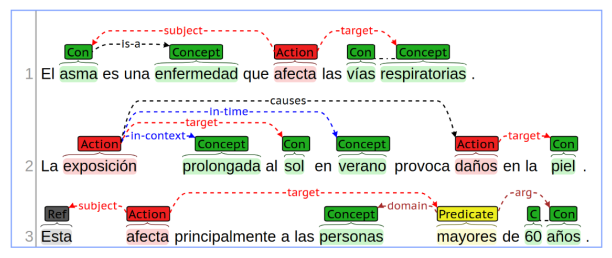
\includegraphics[width=0.9\linewidth]{Graphics/relations.png}
	\caption{Anotación de las relaciones semánticas relevantes en un conjunto de oraciones de ejemplo.} \label{fig:relations_ex}
\end{figure}


\subsection{Escenarios de Evaluación}\label{subsec:eval_sce}

El concurso propone un escenario de evaluación principal (Escenario 1) donde las dos tareas descritas anteriormente se realizan de forma secuencial.
La entrega que obtiene el puntaje F1 más alto para el Escenario 1 es
considerada el sistema con mejor rendimiento general en el concurso.
Adicionalmente, los participantes tuvieron la oportunidad de enfocarse en una de las dos tareas específicamente, a partir de entregar resultados en dos escenarios opcionales, uno para cada tarea.
Estos dos escenarios adicionales miden el rendimiento en tareas individuales de forma independiente entre ellas.

\begin{description}
	
\item[Escenario 1 [A+B]:] Recibe como entrada un conjunto de oraciones a anotar.
El sistema produce tanto las instancias concretas de entidades
presentes en la colección como las relaciones existentes entre ellas.
El rendimiento general del sistema se mide en función
del rendimiento en ambas tareas, según se describe en la sección 4.1.2.
 
\item[Escenario 2 [A]:] Recibe como entrada un conjunto de oraciones a anotar.
El sistema produce únicamente el conjunto de entidades presentes en la colección (con la correspondiente clasificación según el tipo de concepto que representa).

\item[Escenario 3 [B]:] Recibe como entrada un conjunto de oraciones y una colección de entidades anotadas y etiquetadas en el texto.
El sistema produce únicamente el conjunto de relaciones que existen entre las instancias concretas de los conceptos.

\item[Escenario 4 [A+B~(Dominio General)]:] Este escenario fue incluido como una novedad en el evento del año 2020.
Es similar al Escenario 1 de evaluación, pero considera oraciones cuyo contenido es de dominio general.

\end{description} 

El Escenario 1 es considerado más complejo que solucionar cada escenario opcional por separado, dado que los errores que generen los sistemas al enfrentar la Tarea A son transmitidos a la Tarea B.
Por esta razón, es considerado el principal medio de evaluación.

\subsection{Métricas de Evaluación}

La métrica de evaluación es la medida \textit{F1} estándar, donde la precisión y recobrado se definen en términos de coincidencias \textbf{[C]orrectas}, \textbf{[I]ncorrectas},
\textbf{[P]arciales}, \textbf{[F]altantes} y \textbf{[S]obrantes}.


\begin{description}
	
	\item[Anotación correcta:] Reportada cuando una palabra clave es encontrada cuya sección de texto (secuencia de tuplas \texttt{<INICIO, FIN>}) coincide	exactamente con la de una en el corpus de referencia.
	Solo una coincidencia correcta por entrada en la colección de referencia puede ser reportada.
	Por tanto, las entradas duplicadas cuentan como Sobrantes.
	
	\item[Anotación incorrecta:] Reportada cuando una entidad es identificada correctamente en lo que a sección de texto respecta, pero no le fue asignado el tipo de concepto correcto.
	
	\item[Anotación parcial:] Reportada cuando dos intervalos \texttt{<INICIO, FIN>} tienen una intersección no vacía, como es el caso de “vías respiratorias”	y “respiratorias”.
	Notar que una anotación parcial es considerada solo sobre una única anotación correcta en la colección de referencia.
	
	\item[Anotación faltante:] Aquellas anotaciones que aparecen en la colección de	referencia pero no en la respuesta.
	
	\item[Anotación sobrante:] Aquellas anotaciones que aparecen en la respuesta pero no en la colección de referencia.
	
\end{description}

Una mayor precisión significa que el número de anotaciones sobrantes
es menor que el número de anotaciones faltantes, y un mayor recobrado significa lo opuesto.
A las coincidencias parciales se les asigna la mitad de la
puntuaciones de las coincidencias correctas, mientras que a las anotaciones faltantes y sobrantes no se les da puntos.
Las fórmulas de evaluación para el Escenario 1 se definen de la siguiente forma:

\begin{equation*}
P = \frac{C_A + \frac{1}{2}P_A + C_B}{C_A + I_A + P_A + S_A + C_B + S_B}
\end{equation*}

\begin{equation*}
R = \frac{C_A + \frac{1}{2}P_A + C_B}{C_A + I_A + P_A + F_A + C_B + F_B}
\end{equation*}

\begin{equation*}
F1 = 2\frac{PR}{P+R}
\end{equation*}

Siendo $P$ y $R$ los valores de precisión y recobrado respectivamente.

Análogamente, se definen fórmulas similares para los escenarios 2 y 3, pero usando solo las estadísticas de la tarea A y B, respectivamente.

\subsection{Corpus de Evaluación}


\subsection{Implementación y Bibliotecas Externas}

La implementación de las propuestas se realizó utilizando el lenguaje de programación Python.
Se utilizó la biblioteca \texttt{PyTorch} como marco para el trabajo con redes neuronales profundas.
Para la obtención de los \textit{embedding} contextuales se utilizó una variente del modelo \texttt{BERT}~\cite{devlin2018bert}, en este caso: \texttt{bert-base-multilingual-uncased}, a través de la interfaz que brinda la biblioteca \texttt{pytorch-pretrained-bert}~\footnote{https://pypi.org/project/pytorch-pretrained-bert/}.
Los \textit{embeddings} de palabras fueron entrenados utilizado el algoritmo \texttt{word2vec}~\cite{mikolov2013efficient} con la arquitectura \texttt{skipgram}, utilizando la interfaz de la biblioteca \texttt{gensim}~\footnote{https://pypi.org/project/gensim/}.
Las etiquetas de POS-tag así como el árbol de dependencias fueron obtenidos utilizando la biblioteca \texttt{spaCy}~\footnote{https://spacy.io/}.

\subsection{Infraestructura Computacional}



\subsection{Entrenamiento y Ajuste de Parámetros}

Los algoritmos definidos para la resolución de ambas tareas, están basados en técnicas de aprendizaje profundo.
Una de las implicaciones de esta decisión, es que una vez fijo el algoritmo, existe una amplia variedad de hiperparámetros que se pueden ajustar en virtud de obtener mejores resultados computacionales.

Las tablas \ref{table:params_taskA} y \ref{table:params_taskB} describen las configuraciones de parámetros utilizadas cada uno de los modelos y para su entrenamiento.

\begin{table*}[tb]\centering
		\begin{tabular}{lc}
			\hline
			\textbf{Parámetro} & \textbf{Valor} \\
			\hline
			\hline
			\multicolumn{2}{c}{\textbf{Entradas}}\\
			\hline
			\hline
			Dim. del \textit{embedding} contextual & 9216~(12 capas)\\
			Dim. del \textit{embedding} de palabras & 300\\
			Dim. del \textit{embedding} de caracteres & 100\\
			Dim. del \textit{embedding} de POS-tag & 100\\
			
			\hline
			\hline
			\multicolumn{2}{c}{\textbf{Red neuronal}}\\
			\hline
			\hline
			
			Dimensión de la BiLSTM & 300\\
			
			\hline
			\hline
			\multicolumn{2}{c}{\textbf{Entrenamiento}}\\
			\hline
			\hline
			
			Optimizador & Adam\\
			\textit{Learning rate} & 0.001\\
			Épocas & 20\\
			
			\hline
			
		\end{tabular}
	
	\caption{Configuración de parámetros del modelo de extracción de entidades. \textbf{[Arriba]} Red neuronal. \textbf{[Abajo]} Entrenamiento.}\label{table:params_taskA}
	
\end{table*}

\begin{table*}[tb]\centering
	\begin{tabular}{lc}
		\hline
		\textbf{Parámetro} & \textbf{Valor} \\
		\hline
		\hline
		\multicolumn{2}{c}{\textbf{Entradas}}\\
		\hline
		\hline
		Dim. del \textit{embedding} contextual & 768~(última capa)\\
		Dim. del \textit{embedding} de palabras & 300\\
		Dim. del \textit{embedding} de caracteres & 50\\
		Dim. del \textit{embedding} de POS-tag & 50\\
		Dim. del \textit{embedding} de dependencias & 50\\
		Dim. del \textit{embedding} de las etiquetas BMEWO-V & 50\\
		Dim. del \textit{embedding} del tipo de entidad & 50\\
		
		\hline
		\hline
		\multicolumn{2}{c}{\textbf{Red neuronal}}\\
		\hline
		\hline
		
		Dimensión de la BiLSTM & 100\\
		Dimensión de la Tree-LSTM & 50\\
		
		\hline
		\hline
		\multicolumn{2}{c}{\textbf{Entrenamiento}}\\
		\hline
		\hline
		
		Optimizador & Adam\\
		\textit{Learning rate} & 0.001\\
		Épocas & 30\\
		Muestreo negativo & 300\% de ej. positivos\\
		
		\hline
		
	\end{tabular}
	
	\caption{Configuración de parámetros del modelo de extracción de relaciones. \textbf{[Arriba]} Red neuronal. \textbf{[Abajo]} Entrenamiento.}\label{table:params_taskB}
	
\end{table*}
		
El entrenamiento de los modelos fue acompañado de un procedimiento de validación cruzada, que permitió determinar un número conveniente de épocas de entrenamiento, ajustar la complejidad de los modelos, así como seleccionar los más efectivos para someterlos a evaluación.


\section{Resultados Computacionales}

Se recogen en este estudio los resultados para los distintos escenarios de evaluación descritos en la subsección \ref{subsec:eval_sce}.
Se analizaron las curvas de aprendizaje para medir el impacto que tiene en la efectividad el tamaño del conjunto de datos utilizado.
Con el objetivo de medir la influencia de las representaciones distribuidas empleadas, se realizó un análisis ablasivo sobre las distintas componentes de la entrada de los modelos.
En el caso del modelo para la extracción de relaciones, se evaluaron adicionalmente las hipótesis sobre el árbol de dependencias.

\subsection{Resultados por Escenarios de Evaluación}

\subsection{Curvas de Aprendizaje}

\subsection{Análisis Ablasivo}

\subsection{Hipótesis del Árbol de Depedencias}

Para ello se entrenó un modelo con una complejidad semejante en términos de parámetros.
Se sustiuyó el camino en el árbol de dependencias por la secuencia de palabras de la oración completa, y se cambió el procesamiento mediante Tree-LSTM del subárbol relevante a las entidades, por una codificación basada en BiLSTM de las palabras que forman parte de las mismas.


\section{Discusión}
%===================================================================================